% Generated by refresh_charts.py from audited result snapshots.
\expandafter\def\csname tpp:OneSampleADE\endcsname{0.857}
\expandafter\def\csname tpp:BudgetReduction\endcsname{62}
\expandafter\def\csname tpp:ETHMin\endcsname{0.600}
\expandafter\def\csname tpp:ZaraTwoMin\endcsname{0.222}
\expandafter\def\csname tpp:MaxSeedSD\endcsname{0.023}
\expandafter\def\csname tpp:NoiseDominantFolds\endcsname{5}
\expandafter\def\csname tpp:UnivRuntime\endcsname{153.7}
\expandafter\def\csname tpp:UnivPreprocess\endcsname{143.6}

\providecommand{\TppInsight}[1]{\csname tpp:#1\endcsname}
\begin{frame}{Trajectron++ samples futures from visible histories}
\noindent{\small\bfseries\color{Teal} LI JUNHAO / MODEL IMPLEMENTATION}\par\medskip
\begin{tikzpicture}[
  stage/.style={draw=Rule,fill=Wash,rounded corners=3pt,minimum height=1.38cm,
    text width=2.72cm,align=left,inner sep=0.14cm,anchor=west,font=\small}
]
\node[stage] (history) at (0,0)
  {\textcolor{Teal}{\bfseries 01 / History}\\Target + 3\,m\\neighbor graph};
\node[stage] (latent) at (3.51,0)
  {\textcolor{Teal}{\bfseries 02 / Latent}\\25-category\\latent prior};
\node[stage] (decode) at (7.02,0)
  {\textcolor{Teal}{\bfseries 03 / Motion}\\GRU predicts\\2D velocity};
\node[stage] (paths) at (10.53,0)
  {\textcolor{Teal}{\bfseries 04 / Paths}\\Integrate to 20\\metric forecasts};
\draw[-stealth,Teal] (history.east) -- (latent.west);
\draw[-stealth,Teal] (latent.east) -- (decode.west);
\draw[-stealth,Teal] (decode.east) -- (paths.west);
\end{tikzpicture}

\vspace{0.55cm}
\begin{columns}[T,onlytextwidth]
\column{.59\textwidth}
{\bfseries\color{Teal} Causal input gate}\par\smallskip
Compute motion within the observed window. Changing future target or
neighbor positions leaves same-seed forecasts identical.
\column{.35\textwidth}
{\bfseries\color{Teal} Audited evidence}\par\smallskip
15 trained runs, validation-only selection and 90 test bundles.
\end{columns}
\end{frame}

% Sampling values come from evidence/sample_budget.csv.
% Fold differences match the Clean forecasts section of submission/FINAL_REPORT.md.
\begin{frame}{Clean performance varies with sample budget and scene}
\begin{columns}[T,onlytextwidth]
\column{.44\textwidth}
{\small\bfseries\color{Teal} Trajectron++ sampling}\par\smallskip
{\small
\setlength{\tabcolsep}{3pt}
\renewcommand{\arraystretch}{1.12}
\begin{tabular*}{\linewidth}{@{\extracolsep{\fill}}rrr@{}}
\toprule
Draws \(K\) & minADE (m) & meanADE (m) \\
\midrule
1  & \TppInsight{OneSampleADE} & \TppInsight{OneSampleADE} \\
5  & 0.484 & 0.855 \\
10 & 0.394 & 0.856 \\
20 & \ModelMetric{trajectronpp}{clean_0}{min_ade_mean} & \ModelMetric{trajectronpp}{clean_0}{mean_ade_mean} \\
\bottomrule
\end{tabular*}\par
}
\smallskip
{\footnotesize\color{Muted} Prefixes of the same clean forecasts.
Equal weight per scene.}\par
\smallskip
{\small\bfseries\color{Teal} \(K=1\) to 20 cuts minADE by \TppInsight{BudgetReduction}\%.}

\column{.52\textwidth}
{\small\bfseries\color{Teal} Trajectron++ vs.\ Social-GAN at \(K=20\)}\par\smallskip
{\small
\setlength{\tabcolsep}{3pt}
\renewcommand{\arraystretch}{1.12}
\begin{tabular*}{\linewidth}{@{\extracolsep{\fill}}lrrr@{}}
\toprule
Scene & \(\Delta\)minADE & \(\Delta\)minFDE & \(\Delta\)ES \\
\midrule
ETH   & \( -0.032 \) & \( -0.196 \) & \( -0.046 \) \\
Hotel & \( +0.069 \) & \( +0.087 \) & \( +0.036 \) \\
Univ  & \( -0.021 \) & \( -0.046 \) & \( -0.036 \) \\
Zara1 & \( +0.005 \) & \( -0.012 \) & \( -0.038 \) \\
Zara2 & \( +0.017 \) & \( +0.039 \) & \( -0.005 \) \\
\bottomrule
\end{tabular*}\par
}
\smallskip
{\footnotesize\color{Muted} Same clean windows. Differences average three paired seeds.
Negative differences (m) favor Trajectron++. ES is Energy Score.}\par
\smallskip
{\small\bfseries\color{Teal} Lower minFDE on 3/5 scenes and ES on 4/5.}
\end{columns}
\end{frame}

\begin{frame}{Even 5\,cm noise hurt more than two missing points}
\centering
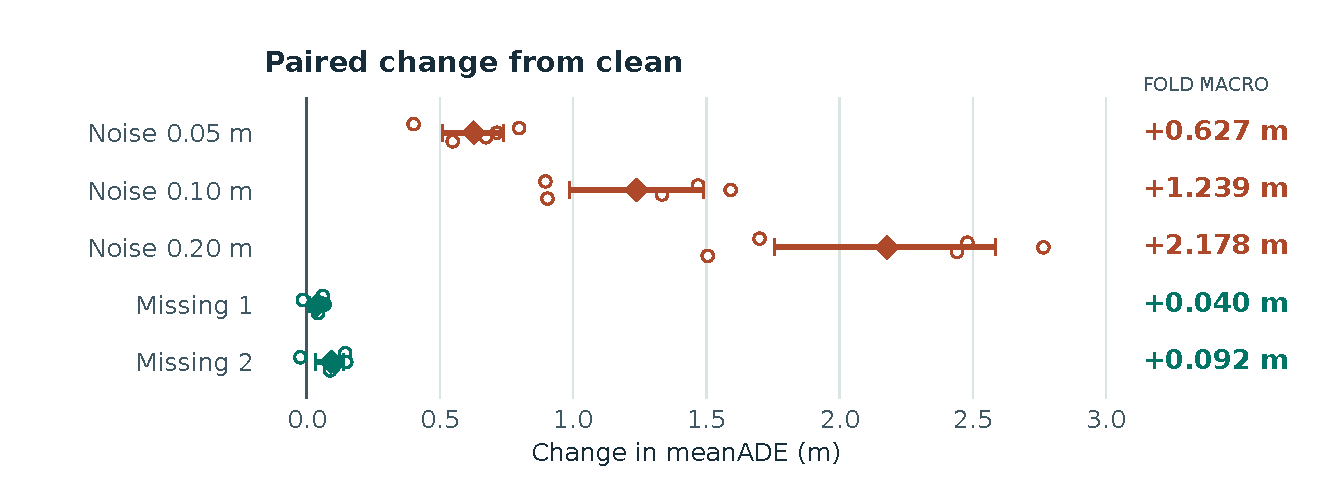
\includegraphics[width=.94\linewidth]{contributions/trajectronpp/assets/paired_robustness.pdf}

\begin{minipage}{.91\linewidth}
\small
\textcolor{Teal}{\bfseries \TppInsight{NoiseDominantFolds}/5 held-out scenes.}
Open circles show scenes. Diamonds and bars show macros and descriptive
95\% intervals. Neighbor histories stay visible.
\end{minipage}
\end{frame}
